\section{Introduction}
\label{intro}

\begin{center}$\vdots$\end{center}

As a motivating example, we consider the Simplified Gap problem.
An intelligent agent is given two strings $x$ and $y$, and is requested
to make them equal by deleting the characters at index range $[i..j)$
from $x$, at a cost of $w_{ij}$ ($0\leq i<j\leq |x|$), from $y$,
at a cost of $w'_{ij}$ ($0\leq i<j\leq |y|$), or by repeating these steps
an arbitrary number of times.
\footnote{In the full version of the gap problem, the agent is also allowed to replace a character $\alpha$ with a character $\beta$, at some cost $c_{\alpha\beta}$.}

The optimal cost is given by the following recurrence:

\begin{equation}
\renewcommand\arraystretch{1.5}
\begin{array}{l@{}l}
	G_{ij} ~=~  &
	\begin{cases}
		0                        & i=j=0 \\
		w_{0j}                   & i=0, j>0 \\
		w'_{i0}                  & i>0, j=0 \\
		\begin{array}{@{}l@{~}l}
		  \min\langle & \underset{0\leq q<j}\min ~ G_{iq} + w_{qj}, \\
		              & \underset{0\leq p<i}\min ~ G_{pj} + w'_{pi}~\rangle
		\end{array}              & i,j>0
	\end{cases}
\end{array}
\label{intro:gap spec}
\end{equation}

\smallskip\noindent
where the desired value is $G_{|x||y|}$.

\medskip
With standard dynamic programming, this recurrence can be computed
with an iterative program, by understanding the dependency pattern:
each value $G_{ij}$ is computed from other values $G_{i'j'}$ with lower
indexes, $i'<i$, ~$j'<j$. Therefore, considering $G$ as a two-dimensional
array, it can be filled in a single pass from left to right and from top
to bottom.

\newcommand\FORLINE[1]{\STATE\algorithmicfor~{#1} \algorithmicdo~}

\begin{algorithm}
\renewcommand\arraystretch{1.3}
\begin{algorithmic}
  \STATE $G_{00} := 0$
  \FORLINE{$j=1..|y|$}  $G_{0j} := w_{0j}$  
  \FOR{$i=1..|x|$}
    \STATE $G_{i0} := w'_{i0}$
    \FOR{$j=1..|y|$}
      \STATE $G_{ij} :=
        \begin{array}[t]{@{}l@{~}l} 
          \min\langle & \underset{0\leq q<j}\min ~ G_{iq} + w_{qj}, \\
                      & \underset{0\leq p<i}\min ~ G_{pj} + w'_{pi}~\rangle 
        \end{array}$
    \ENDFOR
  \ENDFOR
\end{algorithmic}
\end{algorithm}

The same intuition underlies the divide-and-conquer approach for making
a parallel version of the same computation. The array $G$ is partitioned into
quadrants and dependencies are observed at the level of quadrants. The same reasoning
has to be repeated at a coarser level;
so, say the quadrants are labeled 1, 2, 3, and 4, then the computations of 2 and 3 depend on 1,
and the computation of 4 depends on 2 and 3.

\newcommand\qbox[1]{\fbox{\scriptsize#1}}

\begin{figure}[b]
$\renewcommand\arraystretch{2}G ~=~
 \begin{array}{|@{\quad}c@{\quad}|@{\quad}c@{\quad}|} \hline 1 & 2 \\[1mm] \hline 3 & 4 \\[1mm] \hline\end{array}$
\qquad
$\begin{array}{l}\qbox1 \rightsquigarrow \qbox2 \\ 
\qbox1 \rightsquigarrow \qbox3 \\ \qbox2\rightsquigarrow \qbox4 \\ \qbox3 \rightsquigarrow \qbox4\end{array}$
\end{figure}

\medskip
The algorithm designer then writes the following pseudo-code:

\begin{algorithmic}[1]
  \STATE Compute \qbox1 (using only input data $w,w'$).
  \STATE Compute \qbox2 using data from \qbox1.
  \STATE Compute \qbox3 using data from \qbox1.
  \STATE Compute \qbox4 using data from \qbox2 and \qbox3.
\end{algorithmic}

We say that the computation is \newterm{stratified},
in the sense that information flows only in one direction. It can be depicted as
a sequence of steps, each of which reads some regions from the array (possibly none)
and writes into a target region. It can be viewed as a chain, like the one in
\Cref{intro:chain}.

\begin{figure}
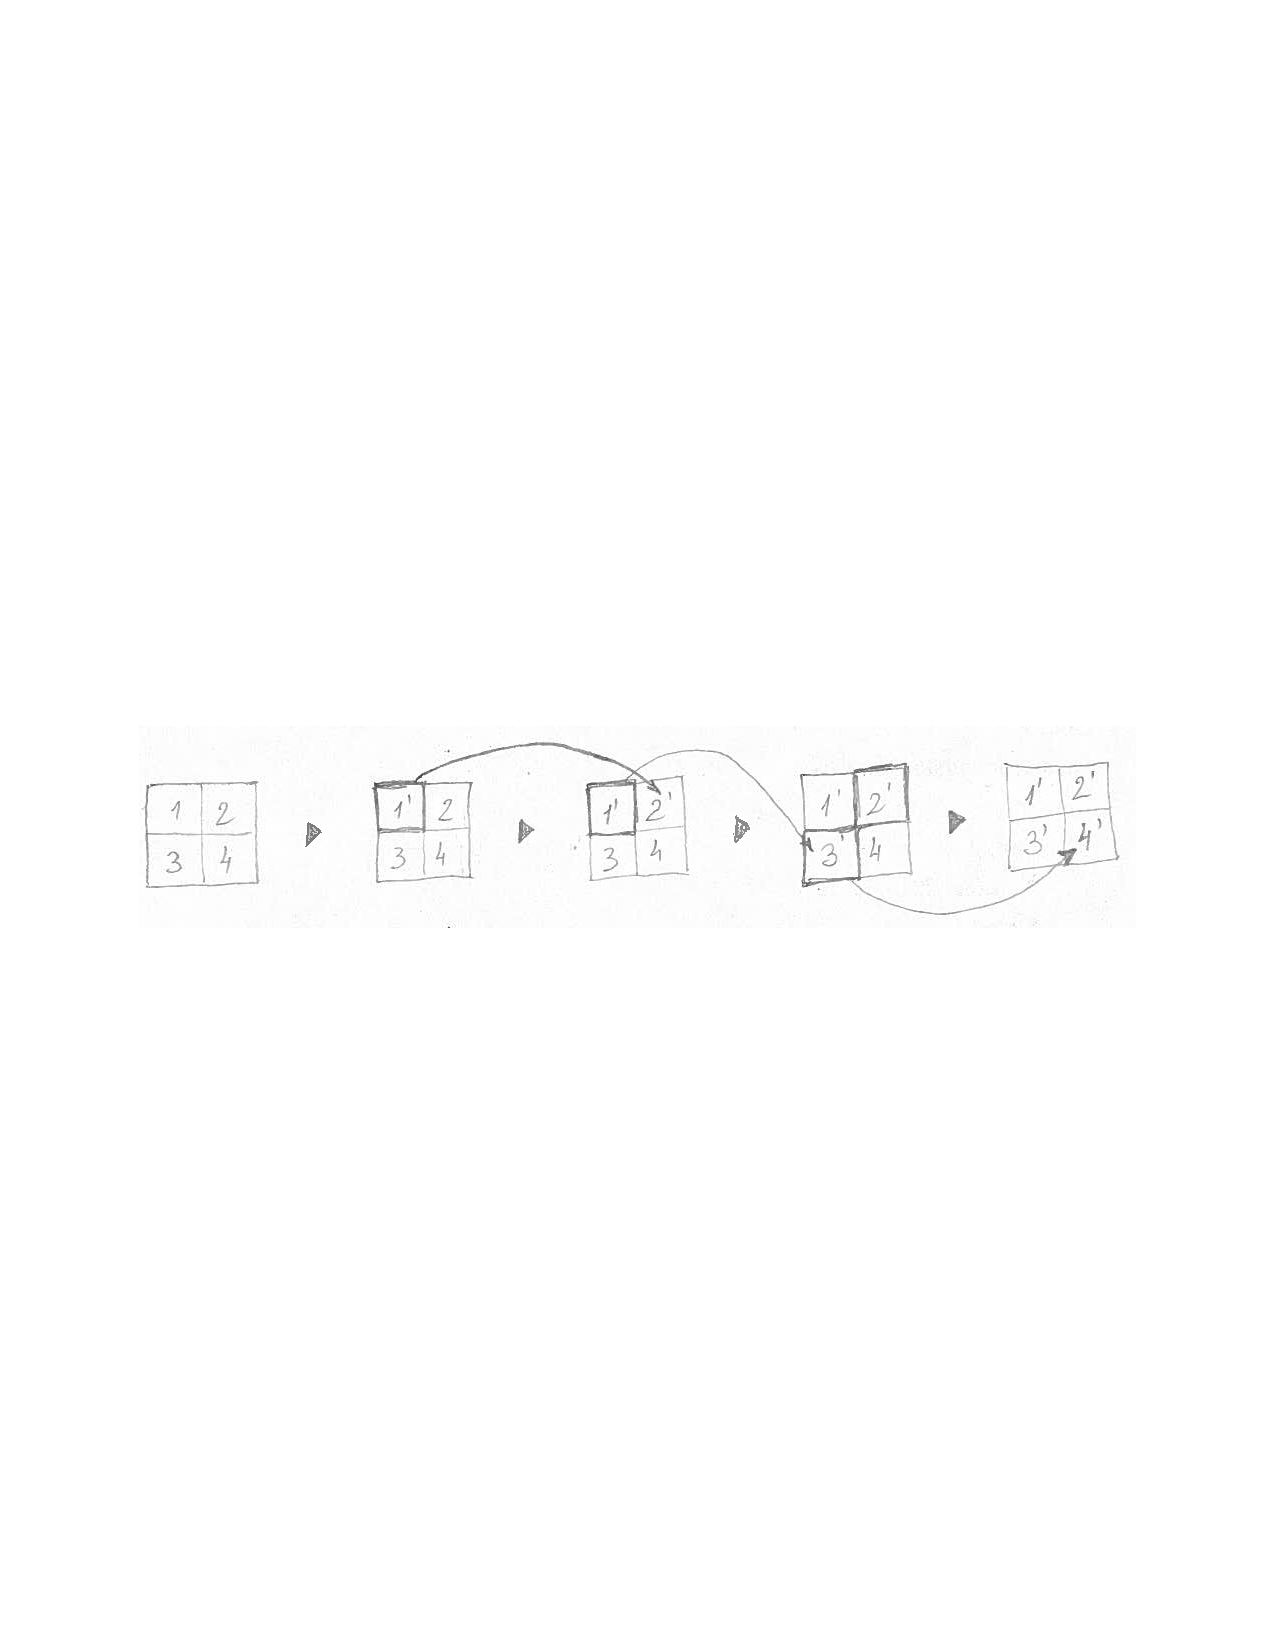
\includegraphics[width=.47\textwidth]{img/gap-stratify1}
\caption[caption]{\label{intro:chain}
  Stratified computation for Simplified Gap. \\[.2em]
  Thick borders indicate the region that is read at each step.}
\end{figure}

At this point it can be noticed that step 1 is equivalent to the original
algorithm when given as input the prefixes of $x$ and $y$ whose length correspond to the
height and width of \qbox1.

With the other three steps, however, things are not so simple:
each of them is required to process some data in addition to the input.
For example, step 2 is required to read values from \qbox1, due to the expression
$G_{iq}$ (where $\scriptstyle 0\leq q<j$).
In order to reason more formally, we define $J$ and $K$ the index sets of the rows
and columns, respectively; $J_0$, $J_1$ for the top and bottom row indexes, respectively;
and $K_0$, $K_1$ for the left and right column indexes (\Cref{intro:slice G}).
The specifications for step 2 then take the following form:

\begin{figure}
\[
\renewcommand\arraystretch{2}
\begin{array}{c|c|c|c|}
  \multicolumn{2}{c}{} & \multicolumn{2}{c}{K} \\ \cline{3-4}
  \multicolumn{2}{c}{} & \multicolumn{1}{c}{K_0}  & \multicolumn{1}{c}{K_1}\\ \cline{3-4}
  \multirow{2}{*}{$J$} & J_0 & 1 & 2 \\ \cline{3-4}
    & J_1 & 3 & 4 \\ \cline{3-4}
\end{array}
\]
\caption{\label{intro:slice G}
  Addressing quadrants in a two-dimensional array.}
\end{figure}

\makeatletter
\newcommand{\LeftEqNo}{\let\veqno\@@leqno}
\makeatother

\begin{equation}\LeftEqNo
\renewcommand\arraystretch{1.5}
\begin{array}{l@{}l}
	G_{\,(i :: J_0)\,(j :: K_1)} ~=~  \\
	\qquad
	\begin{cases}
		0                        & i=j=0 \\
		w_{0j}                   & i=0, j>0 \\
		w'_{i0}                  & i>0, j=0 \\
		\begin{array}{@{}l@{~}l}
		  \min\langle & \underset{0\leq (q::K) <j}\min ~ G_{iq} + w_{qj}, \\
		              & \underset{0\leq (p::J_0) <i}\min ~ G_{pj} + w'_{pi}~\rangle
		\end{array}              & i,j>0
	\end{cases}
\end{array}
\end{equation}

\medskip
Type annotations have been placed on $i$, $j$, $p$, and $q$ to define the regions
over which they range. $i::J_0, j::K_1$ means that the element $G_{ij}$
is always in \qbox2. Similarly, $G_{pj}$ is also in \qbox2. $G_{iq}$ is either in
\qbox1 or in \qbox2.

\begin{figure}
\begin{tabular}{l}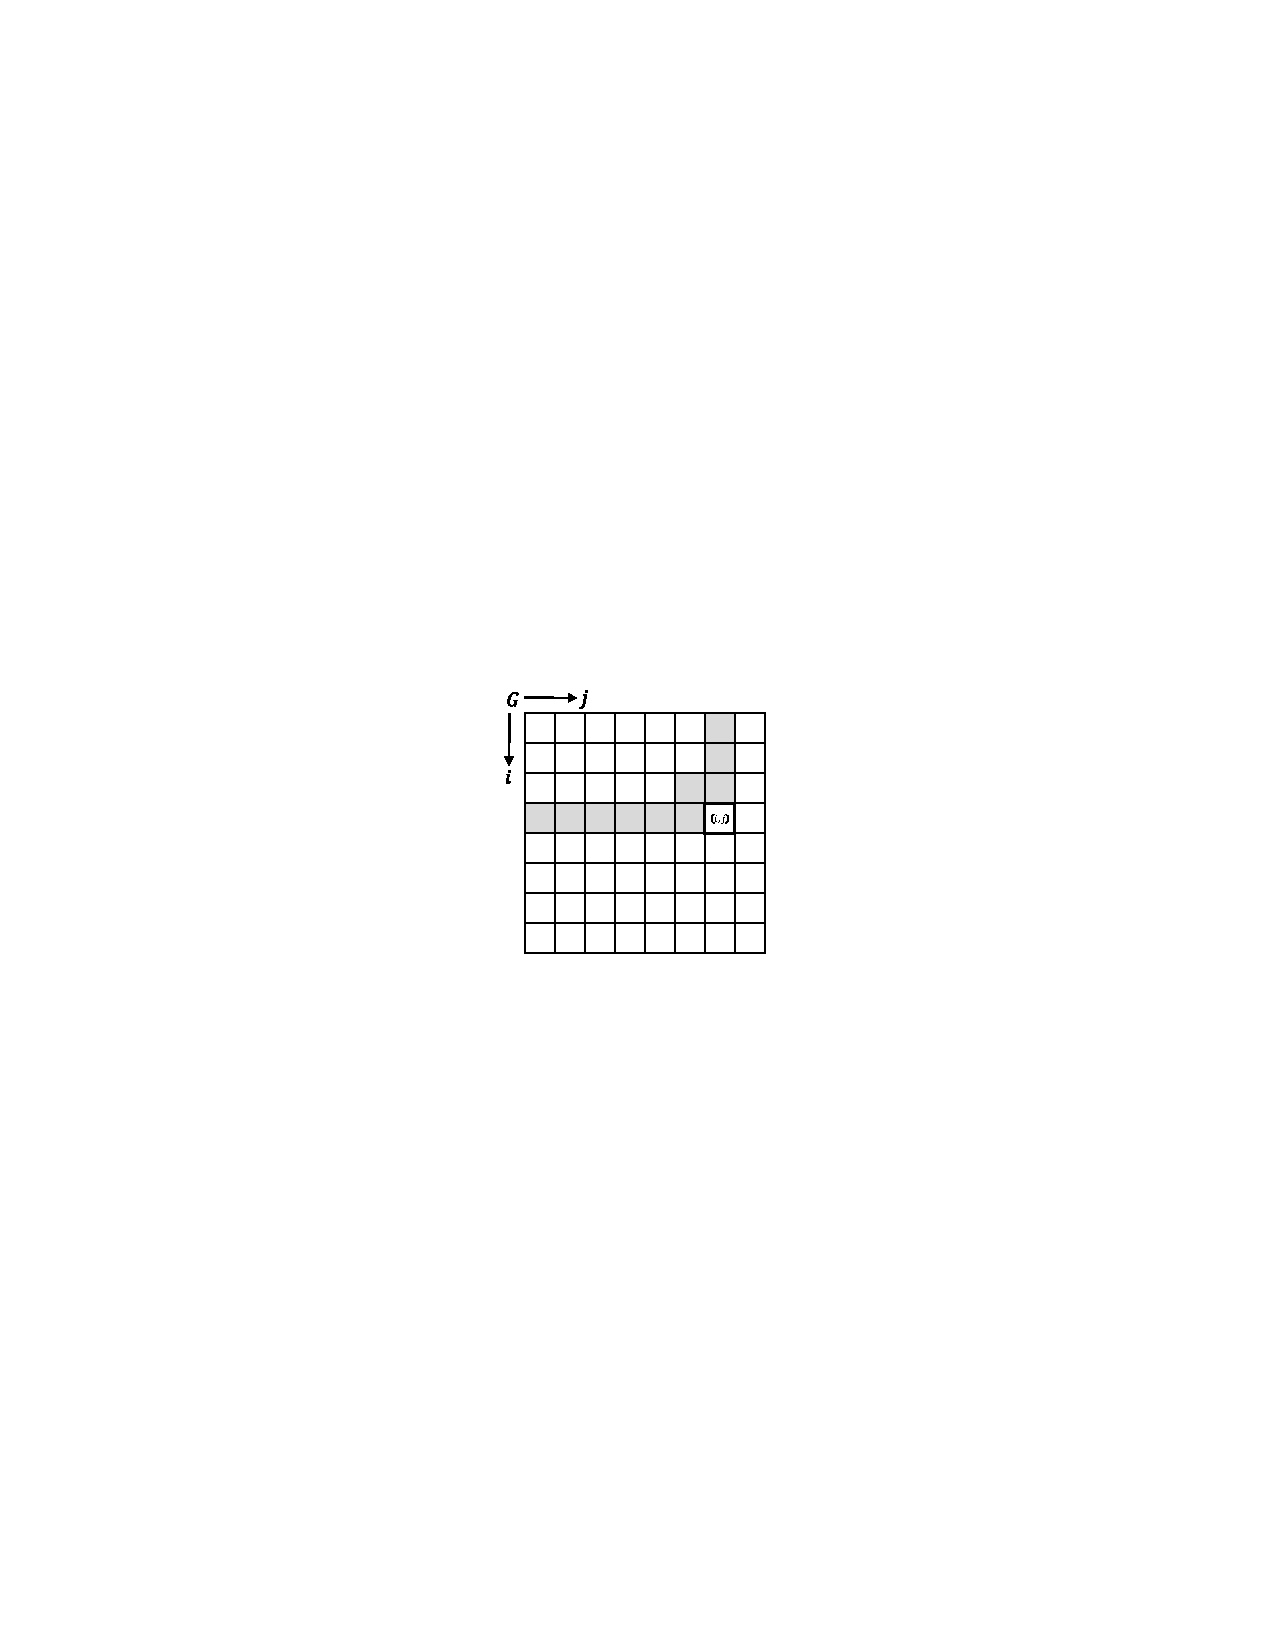
\includegraphics{img/gap-depend}\end{tabular}
\todo{for the simplified version, the cell (i-1,j-1) should not be grayed}
\caption{\label{intro:gap dependency matrix}}
\end{figure}

To address the situation, the algorithm designer would like to separate the parts
of the computation that read from \qbox1 from the parts that read from \qbox2.
This can be achieved here by splitting the $\min_{0\leq(q::K)<j}$ into two
ranges, according to the region in which $G_iq$ resides.

\begin{equation}\LeftEqNo
\renewcommand\arraystretch{1.5}
\begin{array}{l@{}l}
	G_{\,(i :: J_0)\,(j :: K_1)} ~=~  \\
	\qquad
	\begin{cases}
		0                        & i=j=0 \\
		w_{0j}                   & i=0, j>0 \\
		w'_{i0}                  & i>0, j=0 \\
		\begin{array}{@{}l@{~}l}
		  \min\langle & \underset{(q::K_0)}\min ~ G_{iq} + w_{qj}, \\
		              & \underset{(q::K_1) <j}\min ~ G_{iq} + w_{qj}, \\
		              & \underset{0\leq (p::J_0) <i}\min ~ G_{pj} + w'_{pi}~\rangle
		\end{array}              & i,j>0
	\end{cases}
\end{array}
\end{equation}

The path becomes clear: compute $\min_{(q::K_0)} ~ G_{iq} + w_{qj}$ first, for all $i$, $j$
in \qbox2. Then use the results to compute $G_{ij}$.

\begin{equation}\LeftEqNo
\renewcommand\arraystretch{1.5}
\begin{array}{l@{}l}
	G_{\,(i :: J_0)\,(j :: K_1)} ~=~  \\
	\qquad
	\textrm{let}~\psi_{ij} = \underset{(q::K_0)}\min ~ G_{iq} + w_{qj} \\
	\qquad\textrm{in} \\
	\qquad
	\begin{cases}
		0                        & i=j=0 \\
		w_{0j}                   & i=0, j>0 \\
		w'_{i0}                  & i>0, j=0 \\
		\begin{array}{@{}l@{~}l}
		  \min\langle & \psi_{ij}, \\
		              & \underset{(q::K_1) <j}\min ~ G_{iq} + w_{qj}, \\
		              & \underset{0\leq (p::J_0) <i}\min ~ G_{pj} + w'_{pi}~\rangle
		\end{array}              & i,j>0
	\end{cases}
\end{array}
\label{intro:let in 2}
\end{equation}

\medskip
The second part in \eqref{intro:let in 2} starts to look similar to \eqref{intro:gap spec}:
in particular, the types of $p$ and $q$ are the same as those of $i$ and $j$.
In fact, if we set $\psi_{ij}=\infty$, we get \eqref{intro:gap spec} as a special case,
only with $J_0$ and $K_1$ instead of $J$ and $K$.
It therefore makes sense to write a version that generalizes both.

\begin{equation}\LeftEqNo
\renewcommand\arraystretch{1.5}
\begin{array}{l}
	A_{\,\psi\, (i :: J)\, (j :: K)} ~=~  \\
	\qquad
	\begin{cases}
		0                        & i=j=0 \\
		w_{0j}                   & i=0, j>0 \\
		w'_{i0}                  & i>0, j=0 \\
		\begin{array}{@{}l@{~}l}
		  \min\langle & \psi_{ij}, \\
		              & \underset{(q::K)<j}\min ~ A_{\psi iq} + w_{qj}, \\
		              & \underset{(p::J)<i}\min ~ A_{\psi pj} + w'_{pi}~\rangle
		\end{array}              & i,j>0
	\end{cases}
\end{array}
\label{intro:gap phase A}
\end{equation}

\medskip
And we can now rewrite \eqref{intro:gap spec} and \eqref{intro:let in 2} as
%
\begin{equation}
	G_{ij} ~=~ A_{\,(\infty^{JK})\,(i::J)\,(j::K)}
\end{equation}
%
\begin{equation}
\renewcommand\arraystretch{1.3}
\begin{array}{l@{}l}
	G_{\,(i :: J_0)\,(j :: K_1)} ~=~ 
	& \textrm{let}~\psi_{ij} = \underset{(q::K_0)}\min ~ G_{iq} + w_{qj} \\
	& \textrm{in}~A_{\,\psi\,(i::J_0)\,(j::K_1)}
\end{array}	
\label{intro:let in 2 using A}
\end{equation}

\medskip
It takes a bit more insight to notice that \eqref{intro:let in 2 using A} can be further
generalized into:
%
\begin{equation}
\renewcommand\arraystretch{1.5}
\begin{array}{l@{}l}
	A_{\,\psi\,(i :: J)\,(j :: K)} ~=~  \qquad\mbox{(if $i\in J_0$, $j\in K_1$)}\\
	\qquad
	\textrm{let}~\psi'_{ij} = \min \langle~\psi_{ij}, \underset{(q::K_0)}\min ~ G_{iq} + w_{qj}~\rangle \\
	\qquad\textrm{in}~
	A_{\,\psi'\,(i::J_0)\,(j::K_1)}
\end{array}
\label{intro:let in A}
\end{equation}

That is the core of the divide and conquer method: representing the output as a combination
of smaller instances of the problem, or sub-problems, yielding a solution that is essentially
a recursive routine, or a set of mutually recursive routines. In \eqref{intro:let in A}, the
``let''-expression $\psi'_{ij} = \min \langle~\psi_{ij}, \min_{(q::K_0)} ~ G_{iq} + w_{qj}~\rangle$
is another sub-problem that has to be addressed using the same slicing technique.
Once all the pieces fit together, it is possible to cut the space into arbitrarily small pieces,
that fit nicely in each core's local cache. This greately increases performance, as demonstrated
by~\citneeded{perhaps include a table with exact figures}. 

\begin{center}$\vdots$
\end{center}

\subsection{Main Contributions}

\begin{enumerate}
  \item We develop a small set of tactics that can be used to transform a class of recurrence
  specifications intro equivalent divide-and-conquer programs, that admit parallel cache-local
  implementations, in a principled, systematic manner.
  \item We prove that these tactics are semantics-preserving, assuming some side conditions are met
  at the point when the tactic is applied.
  \item We show that the side conditions can be effectively translated into first-order closed
  formulas, and verified automatically by SMT solvers.
\end{enumerate}

